%\documentclass[ignorenonframetext, compress, 9pt, xcolor=svgnames]{beamer} 
\input{../Config_diapos}
\usepackage{color}
\usepackage{tikz}
\usetikzlibrary{shapes.geometric, arrows}
\usepackage{enumerate}   
\usepackage{multirow}
%\setbeamersize{text margin left=1.5em,text margin right=1.5em} 
%\setbeamersize{text margin left=1.2cm,text margin right=1.2cm} 
\setbeamersize{text margin left=1.5em,text margin right=1.5em} 
%\usepackage{xr}
%\externaldocument{Econometrie1_UGA_P2e}
  \usepackage{eso-pic}
%\newcommand\AtPagemyUpperLeft[1]{\AtPageLowerLeft{%
%\put(\LenToUnit{0.9\paperwidth},\LenToUnit{0.85\paperheight}){#1}}}
%\AddToShipoutPictureFG{
 % \AtPagemyUpperLeft{{\includegraphics[width=1.1cm,keepaspectratio]{logoUGA2020.pdf}}}
%}%

%\setbeamercolor{title}{fg=black}
%\setbeamercolor{frametitle}{fg=black}
%\setbeamercolor{section in head/foot}{fg=black}
%\setbeamercolor{author in head/foot}{bg=Brown}
%\setbeamercolor{date in head/foot}{fg=Brown}
\setbeamertemplate{section page}
{
    \begin{centering}
    \begin{beamercolorbox}[sep=11pt,center]{part title}
    \usebeamerfont{section title}\thesection.~\insertsection\par
    \end{beamercolorbox}
    \end{centering}
}
%\titlegraphic{\includegraphics[width=1cm]{logoUGA2020.pdf}}
\title[Regression linéaire]{\textbf{ \'ECONOM\'ETRIE \\ (UGA, S2)}}
\subtitle{\textbf{CHAPITRE 3:\\ ENDOGÉNÉITÉ ET VARIABLES INSTRUMENTALES(1)}}
\date{\today}
\author{Michal W. Urdanivia\inst{*}}
\institute{\inst{*}UGA, Facult\'e d'\'Economie, GAEL, \\
e-mail:
 \href{
     mailto:michal.wong-urdanivia@univ-grenoble-alpes.fr}{michal.wong-urdanivia@univ-grenoble-alpes.fr}}

%\titlegraphic{\includegraphics[width=1cm]{logoUGA2020.pdf}
%}

\begin{document}

%%% TIKZ STUFF
\usetikzlibrary{positioning}
\usetikzlibrary{snakes}
\usetikzlibrary{calc}
\usetikzlibrary{arrows}
\usetikzlibrary{decorations.markings}
\usetikzlibrary{shapes.misc}
\usetikzlibrary{matrix,shapes,arrows,fit,tikzmark}
\usetikzlibrary{shapes}
\usetikzlibrary{shapes.geometric, arrows}
\tikzset{   
        every picture/.style={remember picture,baseline},
        every node/.style={anchor=base,align=center,outer sep=1.5pt},
        every path/.style={thick},
        }
\newcommand\marktopleft[1]{
    \tikz[overlay,remember picture] 
        \node (marker-#1-a) at (-.3em,.3em) {};%
}
\newcommand\markbottomright[2]{%
    \tikz[overlay,remember picture] 
        \node (marker-#1-b) at (0em,0em) {};%
}
\tikzstyle{every picture}+=[remember picture] 
\tikzstyle{mybox} =[draw=black, very thick, rectangle, inner sep=10pt, inner ysep=20pt]
\tikzstyle{fancytitle} =[draw=black,fill=red, text=white]
\tikzstyle{observed}=[draw,circle,fill=gray!50]

\begin{frame}
\titlepage
\end{frame}
\begin{frame}
 \tableofcontents
    \end{frame}
%\begin{frame}
%\frametitle{Contenu}
%\tableofcontents[pausesections, pausesubsections]
%\end{frame}

%\section{Qu'est-ce que l’économétrie ? A quoi (à qui) ça sert ?}
%\frame{\sectionpage}
%\begin{frame}
%  \tableofcontents  
%\end{frame}

\section{Introduction à la notion de variable instrumentale}
\frame{\sectionpage}
\begin{frame}[allowframebreaks]{Endogénéité et (non-)identification dans un modèle linéaire simple}
\begin{itemize}
\item On considère ici le modèle linéaire le plus simple :
\begin{align}
    y_i &=\alpha_0 +b_0x_i + u_i \  \text{avec} \ \Exp[u_i]:= 0,
    \label{eq1}
\end{align}
mais on considère que l’analyse du PGD indique que $x_i$ est endogène dans ce 
modèle, i.e. que :
\begin{align*}
\Exp[u_i| x_i]\neq 0 &\Rightarrow \Cov[x_i; u_i]\neq 0.
\end{align*}
\item Rappelons que lorsque $x_i$ est exogène et que $\Var[x_i] \neq 0$, on a par l'exogénéité de 
$x_i$:
\begin{align*}
    \Cov[x_i; u_i] = 0 &\Leftrightarrow \Cov[x_i; y_i - \alpha_0 +b_0x_i] =0
     \Rightarrow b_0 = \frac{\Cov[x_i; y_i]}{\Var[x_i]}.
\end{align*}
\item Autrement dit l'exogénéité de $x_i$ permet d'identifier $b_0$(et aussi de $\alpha_0$)
comme une fonction de la distribution des variables observées $y_i$ et $x_i$.
\item Inversement dans la situation que nous considérons dans ce chapitre  $\Cov[x_i; u_i]\neq 0$, 
rend impossible l'identification $b_0$(et aussi celle de $\alpha_0$), et 
la construction d'un estimateur convergent.

\framebreak

\item On peut représenter ce problème en utilisant un
\href{https://en.wikipedia.org/wiki/Causal\_graph}{\textbf{graphe causal}}: 

\begin{figure}[hbt!]
    \centering
    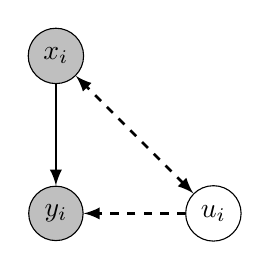
\begin{tikzpicture}
           \node[draw,circle, fill=gray!50](xtilde)  at (0,0) {$x_i$};
          \node[draw,circle,fill=gray!50](y)  at (0,-2) {$y_i$};
      \node[draw,circle](u)  at (2, -2) {$u_i$};
      \draw[->,>=latex, line width= 1] (xtilde) -- (y);
       \draw[->,>=latex, dashed, line width= 1] (u) -- (y);
        \draw[<->,>=latex ,dashed,  line width= 1] (u) -- (xtilde);
          \end{tikzpicture}
          \caption{Graphe causal du modèle: $y_i = \alpha_0 + b_0x_i + u_i$, 
          avec $\Cov(x_i ; u_i)\neq 0$. Les variables
          $(x_i, y_i, u_i)$ sont les nœuds du graph et les 
           nœuds foncés correspondent aux variables observées.
          Les arêtes représentent les relations entre les variables. 
          Les relations observées sont en trait plein.}
    \label{fig1}
          \end{figure}
        \end{itemize}
\end{frame}

\begin{frame}[allowframebreaks]{Identification avec une variable instrumentale}
    \begin{itemize}
\item L'intuition sous-jacente à la méthode des VIs consiste à répondre à la question 
de savoir si avec une variable, que nous notons $z_i$, il est possible d'obtenir 
une mesure de la relation causale entre $x_i$ et $y_i$ qui ne dépende pas de $u_i$.
\item Autrement dit, $z_i$ doit être exogène par rapport à $u_i$:
\begin{align}
\Exp[u_i| z_i] = 0 &\Rightarrow \Cov[z_i; u_i]= 0,
    \label{eq2}
\end{align}
ce qui nous permets d'écrire:
\begin{align*}
    \Cov[z_i; u_i]= 0 &\Leftrightarrow 
    \Cov[z_i; y_i - \alpha_0 +b_0x_i] = 0\\
    &\Leftrightarrow \Cov[z_i; y_i - \alpha_0 +b_0\Cov[z_i;x_i] = 0
\end{align*}
\item Ceci indique que pour identifier $b_0$  on doit aussi supposer aussi que,
\begin{align}
\Cov[z_i;x_i]  &\neq 0,
\label{eq3}
\end{align}
et $b_0$ est identifié par:
\begin{align}
b_0 &= \frac{\Cov[z_i; y_i]}{\Cov[z_i;x_i]},
    \label{eq4}
\end{align}
\framebreak

\item On peut résumer les conditions \eqref{eq2}-\eqref{eq3} ainsi: 

\begin{definition_fr}[Conditions de validité de VIs dans un modèle simple]
    Dans le modèle $y_i = \alpha + b_0x_i + u_i$ avec $\Exp[u_i] := 0$ , une variable $z_i$ 
    est un instrument(de $x_i$) ssi:
    \begin{enumerate}[(i)]
\item $\Cov[z_i ;u_i ]= 0$, i.e. $z_i$ est exogène par rapport à $u_i$ et:
\item $\Cov[z_i;x_i]$, i.e. $z_i$ et $x_i$ sont liées.
\end{enumerate}
\end{definition_fr}

\item Dans la représentation en termes de graphe causal cela donne:

\begin{figure}[hbt!]
    \centering
    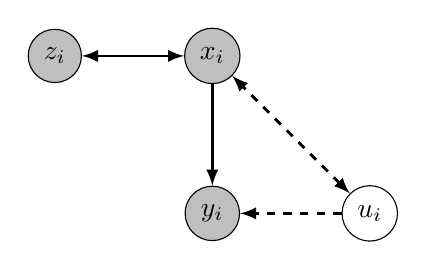
\begin{tikzpicture}
           \node[draw,circle, fill=gray!50](xtilde)  at (0,0) {$x_i$};
           \node[draw,circle,fill=gray!50](ztilde)  at (-2, 0) {$z_i$};
          \node[draw,circle,fill=gray!50](y)  at (0,-2) {$y_i$};
      \node[draw,circle](u)  at (2, -2) {$u_i$};
      \draw[->,>=latex, line width= 1] (xtilde) -- (y);
      \draw[<->,>=latex, line width= 1] (ztilde) -- (xtilde);
       \draw[->,>=latex, dashed, line width= 1] (u) -- (y);
        \draw[<->,>=latex ,dashed,  line width= 1] (u) -- (xtilde);
          \end{tikzpicture}
          \caption{Graphe causal du modèle: $y_i = \alpha_0 + b_0x_i + u_i$, 
          avec $\Cov(x_i ; u_i)\neq 0$, $\Cov(z_i ; u_i) = 0$. Les variables
          $(z_i, x_i, y_i, u_i)$ sont les nœuds du graph et les 
           nœuds foncés correspondent aux variables observées.
          Les arêtes représentent les relations entre les variables. 
          Les relations observées sont en trait plein.}
    \label{fig2}
          \end{figure}

\end{itemize}
\end{frame}
\begin{frame}[allowframebreaks]{Estimateur des VIs dans le modèle simple}
    \begin{itemize}
        \item L'identification de $b_0$ par \eqref{eq4} suggère l'estimateur:
        \begin{align}
            \hat{b}_N^{VI} &= \frac{N^{-1}\sumiN(z_i - \bar{z}_N)(y_i - \bar{y}_N)}{
                N^{-1}\sumiN(z_i - \bar{z}_N)(x_i - \bar{x}_N)} = 
                \frac{N^{-1}\sumiN (z_-\bar{z}_N)y_i}
                {N^{-1}\sumiN (z_-\bar{z}_N)x_i},
                \label{eq5}
        \end{align}
        où $\bar{z}_N$, $\bar{x}_N$, et  $\bar{y}_N$ sont le moyennes empiriques respectives de 
        $z_i$, $x_i$, et $y_i$. 
        \item De plus, $\hat{b}_N^{VI}$ est convergent. Nous avons en effet:
        \begin{align*}
            \underset{N\to + \infty}{\plim} N^{-1}\sumiN (z_-\bar{z}_N)y_i &\rightarrow 
            \Cov[z_i; y_i],\\
            \underset{N\to + \infty}{\plim} N^{-1}\sumiN (z_-\bar{z}_N)x_i &\rightarrow 
            \Cov[z_i; x_i],
        \end{align*}
        d'où:
        \begin{align*}
            \hat{b}_N^{VI} \underset{N\to + \infty}{\limp} 
            \frac{\Cov[z_i; y_i]}{\Cov[z_i;x_i]} &= \frac{\Cov[z_i; \alpha_0 + b_0x_i + u_i]}{\Cov[z_i;x_i]},\\
            &= b_0 + \frac{\Cov[z_i;u_i]}{\Cov[z_i;x_i]},\\
            &=b_0.
        \end{align*}
    \end{itemize}
    \framebreak
    \begin{remark_fr}
        \begin{enumerate}[$\star$]
            \item On dit des variations de $z_i$ qu’elles sont des variations exogènes: 
            elles ne sont pas liées à $u_i$ puisque $\Cov[z_i;u_i]=0$.
            \item Ce sont les effets de ces variations exogènes sur $x_i$ qui sont exploitées pour 
            l’identification de $b_0$ grâce à $\Cov[z_i;x_i]\neq 0$.
            \item Noter qu’il n’est aucunement nécessaire que l’effet de $z_i$ sur $x_i$ soit causal. 
            \item L’effet de $z_i$ sur $y_i$ ne « transite » que via $x_i$. 
            La variable instrumentale $z_i$ n’est pas une variable explicative 
            dans le modèle de $y_i$. 
            On parle alors de relation d’exclusion (de la VI $z_i$ vis-à-vis du modèle de $y_i$). 
            \item L'estimateur des VIs est parfois appelé estimateur des moindres carrés indirects. 
            Cela provient de ce que $b_0$ dans $\eqref{eq4}$ peut s'écrire: 
            \begin{align*}
                b_0 &= \frac{\Cov[z_i; y_i] / \Var[z_i]}{\Cov[z_i;x_i] / \Var[z_i]},
                \end{align*}
            qui est le rapport entre le coefficient de $z_i$ dans la projection de $y_i$ sur $z_i$, 
            et le coefficient de $z_i$ dans la projection de $x_i$ sur $z_i$.
        \end{enumerate}
    \end{remark_fr}
    \end{frame}   
\section{L'estimateur de VIs}
\frame{\sectionpage}
\begin{frame}[allowframebreaks]{Variables endogènes, exogènes, instruments}
\begin{itemize}
    \item L’objectif est maintenant de généraliser l’approche présentée dans
     le cas simple précédent au  modèle linéaire général:
    \begin{align}
        y_i&=\boldx_i^\prime\bolda_0 + u_i, \ \text{avec} \ \Exp[u_i] := 0.
        \label{eq6}
    \end{align}
    \item Plusieurs éléments du vecteur $\boldx_i$ 
    peuvent être endogènes de sorte que dans l'estimateur des MCO de $\bolda_0$ plusieurs
    éléments sont potentiellement biaisés(c.f. cours précédent sur les VIs). 
    \item Notons:

    \[\boldx_i = 
    \begin{bmatrix}
        \begin{bmatrix}
        1\\
        \tilde{\boldx}_i^x
        \end{bmatrix}\\
        \tilde{\boldx}_i^e
    \end{bmatrix} 
    =
    \begin{bmatrix}
        \boldx_i^x\\
        \tilde{\boldx}_i^e
    \end{bmatrix}
    \begin{array}{ll}
        \left\{ \text{variables explicatives exogènes}\right. &: \Exp[u_i|x_{k, i}^x] = 0 (k=1,\ldots,M)\\
        \left\{ \text{variables explicatives endogènes}\right.&: \Exp[u_i|x_{k, i}^x] \neq 0(k=M +1,\ldots,K)
    \end{array}
    \]
    \begin{remark_fr}
    \begin{enumerate}[$\star$]
        \item Il est clair que la variable constante $1$ est «exogène» :$\Exp[1\times u_i] =\Exp[ui|] 
        =\Exp[ u_i] =0$.
        \item Comme pour l'estimateur des MCO nous utiliserons la Méthode des Moments 
        pour construire un estimateur convergent de $\bolda_0$ , l’estimateur des VI 
        du modèle \eqref{eq6}.
        \item On considère ici que chaque élément $\boldx_i^e$ a une variable instrumentale.
    \end{enumerate}
    \end{remark_fr}

    \framebreak
    \begin{definition_fr}[Variable instrumentale]
        $z_{k ,i}$  est une variable instrumentale de $x_{k, i}$ dans le modèle linéaire
         \eqref{eq6} si: 
         \begin{enumerate}[(i)]
            \item $\Cov[z_{k, i}; u_i] = 0$ i.e., $z_{k, i}$ est exogènes par rapport à $u_i$,
            \label{vi1}
            \item $z_{k ,i}$ « suffisamment » liée à $x_{k ,i}$.
            \label{vi2}
         \end{enumerate}
    \end{definition_fr}
    \begin{remark_fr}
        \begin{enumerate}[$\star$]
        \item On verra dans la suite (analyse des conditions de rang) que la condition 
        \eqref{vi2} doit en fait être définie comme:
        \begin{align*}
            \Cov[z_{k, i} ; e_{k, i} ]&\neq 0 \  \text{pour} \ k > 1,
        \end{align*}
        où $e_{k, i}$ est la partie spécifique de $x_{k ,i}$ dans $x_i$ , i.e. 
        le résidu de la projection linéaire de $x_{k ,i}$ sur les autres explicatives $\boldx_{-k, i}$.
        \begin{align*}
            e_{k, i} &= x_{k, i}- \mathcal{EL}[x_{k, i}| \boldx_{-k, i}].
      \end{align*}
      \item Dans la définition d'un VI précédente, on voit que lorsqu'une variable explicative $x_{k, i}$
      est exogène alors c'est aussi une variable instrumentale d'elle même. En ce sens 
      que non seulement elle vérifie \eqref{vi1} mais elle vérifie forcément \eqref{vi2} 
      (car ayant une corrélation de 1 avec elle même)
    \end{enumerate}
    \end{remark_fr}

    \framebreak

    \item On construit le vecteur des variables instrumentales $\boldz_i$ avec:
    
    \[
       \tilde{\boldz}_i^e = 
       \begin{bmatrix} 
        \tilde{z}_{M+1, i}\\
        \tilde{z}_{M+2, i}\\
        \vdots\\
        \tilde{z}_{K, i}
       \end{bmatrix}
       \ \text{et} \
       \boldz_i = 
       \begin{bmatrix}
        \begin{bmatrix}
            1\\
            \tilde{\boldx}_i^x
        \end{bmatrix}\\ 
        \tilde{\boldz}_i^e
       \end{bmatrix}
       = 
       \begin{bmatrix}
        \boldx_i^x\\
        \tilde{\boldz}_i^e
       \end{bmatrix}
       \begin{array}{ll}
        \left\{ \text{variables exogènes de $\boldx_i$}\right.
         &: \Exp[u_i|x_{k, i}^x] = 0 (k=1,\ldots, M)\\
        \left\{ \text{variables instrumentales}\right.&:\Exp[u_i|z_{k, i}] = 0(k=M +1,\ldots,K)
       \end{array}
    \]
    \item Ce vecteur contient en fait toutes les variables exogènes du modèle. Ce sont 
    ces variables qui assurent l’identification des paramètres du modèle.
    \item $\boldz_i$  est parfois nommé ensemble d’information du modèle.


\framebreak 

\begin{definition_fr}[Modèle linéaire à variables instrumentales]
    Le modèle défini par :
    \begin{align*}
        y_i&=\boldx_i^\prime\bolda_0 + u_i, \ \text{avec} \ \Exp[u_i|\boldz_i]= \Exp[u_i]:=0,
    \end{align*}
    est un modèle linéaire à variables instrumentales.
    La condition d’identification de $\bolda_0$ dans ce modèle est donnée par:
    \begin{align*}
    \Rang\left(\Exp[\boldz\boldx^\prime]\right)= K = \dim(\boldx).
\end{align*}
\end{definition_fr}

\begin{remark_fr}
    La condition d’exogénéité de $\boldz_i$ est définie par $\Exp[u_i|\boldz_i]= 0$, et non par 
    $\Cov[\boldz_i ;u_i ]= \boldzero$.
    Ce n’est pas nécessaire pour un modèle linéaire où $\Cov[\boldz_i ;u_i ]= \boldzero$ suffit
    mais c’est standard et cela simplifie la présentation des hypothèses d’homoscédasticité.
\end{remark_fr}

\framebreak

\item Comme dans le cas où on a construit l’estimateur des MCO de a
on part de la condition d’exogénéité des $\boldz_i$ (et non des $\boldx_i$ comme dans le cas
des MCO), i.e. la condition d’orthogonalité donnée par :
\begin{align*}
    \Exp[u_i\boldz_i]=0 &\Rightarrow \Exp[\boldz_iu_i]=0 \Leftrightarrow 
    \Exp[z_i(y_i-\boldx_i^\prime\bolda_0)]=\boldzero.
\end{align*}
\item On a ici la condition de moment estimante pour $\bolda_0$ est $\Exp[\boldz_i(y_i -\boldx_i\bolda_0)]= \boldzero$. 
Et on a alors:
\begin{align*}
     \Exp[\boldz_i(y_i-\boldx_i^\prime \bolda_0)] = \boldzero \Leftrightarrow \bolda = \bolda_0.
\end{align*}
\item On suppose ici que $\bolda_0$ est l’unique solution en $\bolda$ de $\Exp[\boldz_i(y_i-\boldx^\prime\bolda)]= 0$. 
\item Le principe d’analogie définit l’estimateur de la MM de $\bolda_0$ par :
\begin{align*}
    N^{-1}\sumiN \boldz_i(y_i-\boldx_i^\prime\bolda)=\boldzero_{K\times 1} &\Leftrightarrow \bolda = \hat{\bolda}_N^{MM}.
\end{align*}

\item  L’équation dont $\hat{\bolda}_N^{MM}$ est définie comme la solution en $\bolda$ est en fait un système
de $K$ équations linéaires à $K$ inconnues (les éléments de  $\hat{\bolda}_N^{MM}$). 
Il a solution sous forme explicite. On a:
\begin{align*}
    N^{-1}\sumiN \boldz_i(y_i-\boldx_i^\prime\hat{\bolda}_N^{MM})&=\boldzero_{K\times 1}.
\end{align*}
\item Il est aisé de définir la forme de $\hat{\bolda}_N^{MM}$,
\begin{align*}
N^{-1}\sumiN \boldz_iy_i - \left[N^{-1}\sumiN \boldz_i\boldx_i^\prime \right]\hat{\bolda}_N^{MM}&=\boldzero_{K\times 1},
\end{align*}
qui donne finalement :

\begin{align*}
    \hat{\bolda}_N^{MM} &= \left[N^{-1}\sumiN \boldz_i\boldx_i^\prime \right]^{-1}N^{-1}\sumiN \boldz_iy_i,
\end{align*}
qui définit ce qu’on appelle l’estimateur des VI.
\end{itemize}
\end{frame}
\begin{frame}[allowframebreaks]{Références}
\bibliographystyle{jpe}
 \bibliography{../Biblio}
  \end{frame}



    \end{document}
    